\chapter{Suggested Algorithms}
\label{chapter_solutions}

% **************************** Define Graphics Path **************************
\ifpdf
    \graphicspath{{Chapter4/Figs/Raster/}{Chapter4/Figs/PDF/}{Chapter4/Figs/}}
\else
    \graphicspath{{Chapter4/Figs/Vector/}{Chapter4/Figs/}}
\fi

This chapter presents the suggested learning algorithms for predictive models in detail. First section \ref{sec_formalProblemDef} defines the problem of predicting events in a stream formally. Subsequently sections \ref{sec_predictiveEpisodeMining} and \ref{sec_FeatureBasedStreamWindowClassification} explain the two approaches suggested by this thesis, which are called predictive episode rule mining and feature based stream window classification. Finally section \ref{sec_EvolvingModels} explains how the models created by these methods can be evolved as the stream progresses.

\section{Formal Problem Definition}
\label{sec_formalProblemDef}
The problem to be tackled in this thesis is the prediction of future events in data streams using episode patterns. The approaches shall have the following properties:

\begin{itemize}
	\item \textbf{Local and fast prediction:} This thesis does not focus on long term trends or on predictions of special values at fixed times (for example daily closing values of stocks), but instead aim to give predictions about the near future given the current state of the stream.
	\item \textbf{Usage of a Stream of categorical Values} Most forecasting methods focus on regression, meaning the predictions of numerical values. In contrast to these approaches, this thesis will focus on streams of categorical events and aims to predict the occurrences of events of certain types.
\end{itemize}

In this context I define:

\begin{mydef}
\textbf{Categorical Event Stream} A categorical event stream is defined as a (possibly infinite or constantly updating) sequence: $S = [ (T_1,t_1),(T_2,t_2),... ] $ where $T_i \in \Sigma$ is the event type of the i-th event and $t_i \in \mathbb{N}^+$ is the timestamp of the i-th event. The sequence is ordered according to the timestamps, which means that $\forall i,j \in {1,...,n} \; i<j \implies t_i \leq t_j$.
\end{mydef}

Note that this definition is essentially the same as definiton \ref{def_eventSequence}, which defines event sequences. The only difference is that in a categorical event stream new events are allowed to constantly come in, which makes the sequence possibly infinite. Given a categorical event stream it is the goal of this thesis to develop algorithms that will build predictive models:

\begin{mydef}
\label{def_predictiveModel}
\textbf{Predictive Model} A predictive model for $M(T)$, $T \in Sigma$ is a model that if given a window $W$ (see definition \ref{def_timeWindow}) of a categorical event stream will output a binary value in the following:
\begin{itemize}
	\item $1$ if the model expects an event of type $T$ to occur shortly after $W$.
	\item 0 otherwise.
\end{itemize} 
\end{mydef}

Definition \ref{def_predictiveModel} purposefully remains vague about what \textit{"shortly after"} means mathematically, since this may depend on the underlying stream, or the users intent. Usually this will mean something like \textit{"x time units in the future"} or \textit{"at most x time units in the future"}

\section{PERMS - Predictive Episode Rule Mining in Streams}
\label{sec_predictiveEpisodeMining}
The first suggested algorithm is called the PERMS algorithm, short for \textbf{P}redictive \textbf{E}pisode \textbf{R}ule \textbf{M}ining in \textbf{S}treams.

\subsection{Basic Idea}
In order to fully explain the algorithm I first need to define what is meant by predictive episode rules.

\begin{mydef}
\label{def_predictiveEpisode}
\textbf{Predictive Episode Rule} An episode $\alpha$ is called a predictive episode rule for event $A \in \Sigma$ if $\alpha$ has the form $\beta \rightarrow A$ where $\beta$ is an episode. In this context $\beta$ is also referred to as the prefix or predictor and $A$ is referred to as the suffix or target event of $\alpha$. 
\end{mydef}

The basic idea of the prediction algorithm using predictive episode rules is rather simple. If given a set $P$ of predictors, the stream is monitored and whenever a predictor in $P$ is detected the model predicts an occurrence of $A$. The idea is similar to the mining of sequential rules or rule-based classification \cite{ma1998integrating}.
Of course there is an infinite amount of predictive episode rules for an event type, finding those predictive episode rules that are actually useful for predicting the occurrence of an event is the main task when building (training) the model. The use case here is very similar to the related work that deals with the constraint based mining of episode rules \cite{meger2004constraint}, where episode rules are mined in order to discover dependencies between earthquakes. There are two main important differences that make the approach used by the authors impractical:

\begin{itemize}
 \item In order to build predictive models only episode rules of one specific type are of interest (those predicting the desired event $A$). Thus it is not necessary to mine all frequent episode rules in the stream.
 \item This thesis deals with data in a streaming environment, meaning it is impossible to analyze the whole data or make multiple passes over the entire stream.
\end{itemize}

The core concepts of the algorithm that builds the set $P$ revolve around frequency, support and confidence for predictive episode rules, which are similar to the equally named concepts in classic association rule mining \cite{agrawal1994fast}. Before these concepts can be defined for predictive episode rules however, an episode frequency measure needs to be chosen. 

\subsection{Choice of Frequency Measure}

Recall that there are three main frequency measures that were proposed in the literature:

\begin{itemize}
	\item The window-based frequency (see defintion \ref{def_windowBasedFrequency})
	\item The frequency based on minimal occurrences (see definition \ref{def_minimalOccuranceFrequency})
	\item The frequency based on non-overlapping occurrences (see definition \ref{def_nonOverlappingFrequency})
\end{itemize}

Their properties were already briefly discussed in section \ref{sec_otherFrequency}. While the frequency measure using the non-overlapping occurrences is the latest measure and offers the best theoretical runtime, when recognizing episodes in a sequence it has a few drawbacks that are detrimental to its use in the given scenario. The first one is that it does not limit the duration of the episode occurrences. However limiting the duration of episode rules, or in other words giving episode occurrences expiry times is necessary when predicting event occurrences in streams. Consider for example the simple predictive episode rule $\alpha = B \rightarrow A$ and the following example sequence: 

\begin{equation}
S = [ (B,1),(C,2),(A,3),(B,4),...,(A,2000) ] 
\end{equation}

The non-overlapping frequency definition recognizes both $(B,1) \rightarrow (A,3)$ and $(B,4) \rightarrow (A,2000)$ as equally valid occurrences of $\alpha$ in $S$. However it is to be expected that when looking for episode rules for predictive purposes in a stream the events should happen close to each other (time-wise). This means that in this case $(B,1) \rightarrow (A,3)$ is likely a correct occurrence and prediction, whereas the occurrence $(B,4) \rightarrow (A,2000)$ is simply owed to the fact that at some point of time event $A$ will occur again in the stream and $(B,4)$ happened to occur a long time before that, without there necessarily being a correlation or causality.
Additionally the non-overlapping frequency assumes that there is one long sequence, from which the episodes are to be mined. The window-based frequency however works on a set of individual windows of a sequence or stream. In the previous work this had not been an advantage or disadvantage, since it did not focus on the streaming scenario, which meant that it was possible to analyze the entire sequence. This lead to the use of sliding windows over the sequence when using the window-based frequency. In the streaming scenario it is impossible to use all of the data, instead a certain selection is necessary. This can be done easily when using the window-based frequency by simply storing the windows that are of interest. Selecting data for the non-overlapping frequency definition is more difficult. Thus the algorithms suggested in this thesis will use the window-based frequency.

\subsection{Basic Definitions}
Since the frequency measure was decided on it is now possible to define frequency, support and confidence of predictive episode rules.

\begin{mydef}
\label{def_frequency}
\textbf{Frequency} If given a set of time windows $WIN$ (see definition \ref{def_timeWindow}) of a sequence or stream the frequency of a predictive episode rule $\alpha$ is defined as the number of windows in which $\alpha$ occurs: $freq(\alpha,WIN) = |\{W\,|W \in WIN\; \land \alpha\; occurs \; in \; W\}|$
\end{mydef}

\begin{mydef}
\label{def_support}
\textbf{Support} If given a set of time windows $WIN$ of a sequence the support of a predictive episode rule $\alpha$ is defined as $s(\alpha,WIN) = \frac{freq(\alpha)}{|WIN|}$
\end{mydef}

\begin{mydef}
\label{def_confidence}
\textbf{Confidence} If given a set of time windows $WIN$ of a sequence the confidence of a predictive episode rule $\alpha = \beta \rightarrow A$ is defined as $c(\alpha,WIN) = \frac{s(\alpha,WIN)}{s(\beta,WIN)}$ \cite{meger2004constraint}
\end{mydef}

The intention is clear and similar to the mining of classic association rules \cite{agrawal1994fast}: If a rule has a high confidence, it means that the prefix of the rule rarely occurs without its suffix $A$, meaning there is a high chance that this is a true predictor for the event $A$. Thus the goal of PERMS is to find a set of predictors $P$ that have a very high confidence and are above a certain support limit.

\subsection{Choice of Training Data}
Recall that in streaming applications it is impossible to analyze the whole stream as one sequence using multiple passes. Thus, when presented with a stream any prediction or forecasting algorithm first needs to take some time to study the stream and extract training data to build the model. So if given a categorical event stream, how can the training data be selected? As it was described in section \ref{sec_basicEpisodeDefinitions} the data basis for episode mining is one very long sequence. Thus the first simple approach would be to simply record the stream as a sequence until a certain number of desired elements was reached or the machine runs out of memory. The recorded sequence would then be the training sequence from which the predictive episode rules can be mined. This approach is visualized in figure \ref{fig_trainingDataNaive}.

\begin{figure}[h]
	\centering
  	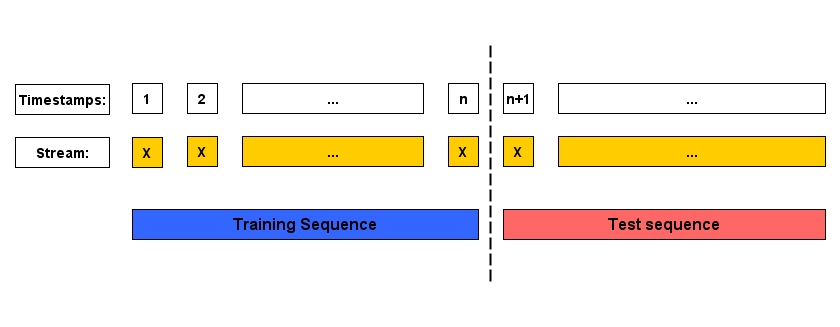
\includegraphics[width=\textwidth]{trainingDataNaive}
	\caption{Visualization of a simple split of the stream into a training segment at the beginning, followed by a (potentially endless) test phase}
	\label{fig_trainingDataNaive}
\end{figure}

The disadvantage of this naive approach is that there is no guarantee about the number of occurrences of the target event. For example if $A$ is the target event and $A$ is rather sparse in the beginning of the stream, then there will be a very small data basis to extract predictive episode rules for $A$ and thus the algorithm will likely not be able to find useful predictive episode rules. 
A better approach is to keep a window of the stream with a certain duration $d$ in memory and scan the stream for occurrences of the target event $A$. Whenever an event of type $A$ enters the window the algorithm stores the current window in a list until there is a sufficient number of windows. This approach is visualized in figure \ref{fig_trainingDataWindowsOfA}. It guarantees that the algorithm will have a sufficient number of windows that are immediately followed by the target event. The mining process then is to simply find frequent episodes in the mined windows. Each of these then automatically corresponds to the prefix of a potential predictive episode rule with the suffix being the target event ($A$ in the figures). The window duration $d$ simultaneously determines the maximum duration for episode occurrences, which is exactly $d$.

\begin{figure}[h]
	\centering
  	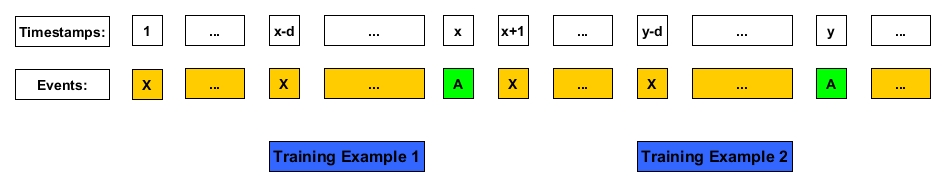
\includegraphics[width=\textwidth]{trainingDataWindowsOfA}
	\caption{Visualization of using fixed windows that precede the target event as training examples. Predictive episodes can be mined from the windows that are extracted from the stream as shown above.}
	\label{fig_trainingDataWindowsOfA}
\end{figure}

The obvious and very big disadvantage of this approach is that there are no negative examples in the training sample taken from the stream. Each window is immediately followed by the target event $A$, thus every episode mined from the windows can have $A$ appended as a suffix and thus every predictive episode rule will have a confidence of $1.0$. This means that selection via confidence is meaningless, since there are no negative examples, meaning windows that are not followed by $A$. However negative examples can be extracted from the stream in a similar manner. This results in $m$ positive examples, also referred to as positive windows, which are followed by $A$ and $m$ negative examples, also called negative windows, which are not followed by $A$. This is the basic idea behind the training data selection in PERMS. It is visualized in figure \ref{fig_trainingDataPositiveAndNegativeWindows}. 

\begin{figure}[h]
	\centering
  	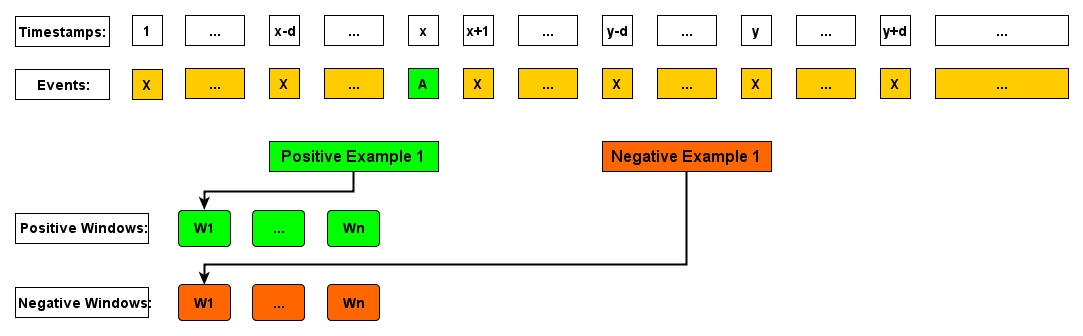
\includegraphics[width=\textwidth]{trainingDataPositiveAndNegativeWindows}
	\caption{Extracting positive and negative example windows from the stream.}
	\label{fig_trainingDataPositiveAndNegativeWindows}
\end{figure}

In order to make sure, that none of the patterns in the negative windows are followed by event $A$, even if they occur right before the end of the window, it is helpful to require that $A$ does not occur after the negative window for the next $d$ time units. This means that the algorithm needs to keep a window of the stream, that has $2\cdot d$ duration.\\
There are still some issues with this approach that can be detrimental to the predictive performance of the model. One issue is that an equal amount of positive and negative windows is extracted from the stream without considering the original distribution. If $A$ occurs very rarely, having an equal amount of positive and negative examples in the training data does not reflect the original event distribution in the stream. If that is the case, this can be fixed by including a number of negative examples that is proportionate to the original distribution (which is either known or learned while extracting the training data). However it is unclear if that would actually have a significantly positive effect on the performance of the resulting model. \\
This approach is actually similar to the approach of Laxman et al. as described in their paper about generative models for prediction in streams \cite{laxman2008stream}. They do however only consider serial episodes and focus on learning hidden markov models in order to predict events, as opposed to finding episode rules.

\subsection{PERMS Parameters and Pseudocode}
\label{subsec_perms}

The PERMS algorithm uses the following user-defined parameters:

\begin{itemize}
	\item \textbf{$d$} - the duration of the sliding window. This also implies that all windows which the predictive episode rules will be mined from will exactly have a duration of exactly $d$ time units.
	\item \textbf{$m$} - the number of positive windows to mine the predictive episode rules from. This means that PERMS will mine $m$ positive and $m$ negative training examples from the stream.
	\item \textbf{$s_P$} - the minimum support that parallel predictive episode rules must have to be considered for the model (parallel episodes with support $s_P$ or higher are frequent).
	\item \textbf{$s_S$} - the minimum support that serial predictive episode rules must have to be considered for the model (serial episodes with support $s_S$ or higher are frequent).
	\item \textbf{$n$} - the desired size of the final set of predictive episodes, also referred to as the ensemble size.
\end{itemize}

The pseudocode for PERMS is given in algorithm \ref{alg_PERMS}. Recall that for formally accessing episodes I use the notation introduced in section \ref{sec_basicEpisodeDefinitions}.

\begin{algorithm}[H]
  \caption{PERMS
    \label{alg_PERMS}}
  \begin{algorithmic}[1]
    \Statex
    \Require Let $S=[(T_s,t_1),...]$ be a stream of events and let $d$,$m$,$s_P$,$s_S$,$n$ be the parameters as defined in the beginning of subsection \ref{subsec_perms}.
    \Function{PERMS}{}
      \Let{$(PE,NE)$}{$WindowMining(S,d,m,A)$} 
      \Let{$P$}{$BuildPredictiveEpisodeModel(PE,NE,s_P,s_S,n)$}
      \State apply set of predictors $P$ to the rest of the stream $S$
    \EndFunction
  \end{algorithmic}
\end{algorithm}

As seen in the algorithm above the basic idea of the PERMS algorithm can be divided into 2 parts: training example mining (window mining) and predictive episode model building. To mine the training examples PERMS starts at the beginning of the stream and keeps a sliding window of a user defined duration $d$ in memory (see definition \ref{def_timeWindow}). Whenever an event of type $A$ enters the window PERMS stores the current window in a list until a sufficient number of windows was reached ($m$). Additionally PERMS also stores $m$ windows that do not contain $A$ and were also not followed by $A$ in the near future. The pseudocode for this is given in algorithm \ref{alg_traningExampleMining}.

\begin{algorithm}[H]
  \caption{Training Example Mining
    \label{alg_traningExampleMining}}
  \begin{algorithmic}[1]
    \Statex
    \Require Let $S=[(T_s,t_1),...]$ be a stream of events, $d$ be the window duration, $m$ the required number of windows and $A$ the event type to predict.
    \Function{WindowMining}{}
      \Let{$PE$}{$\emptyset$} 
      \Let{$NE$}{$\emptyset$}
      \Let{$i$}{$1$}
      \Let{$t_{last}$}{$t_1$}
      \While{$|PE| \neq m \; \lor |NE| \neq m $}
      	\Let{$(T_i,t_i)$}{$S[i]$}
      	\If{$T_i = A$}
      		\Let{$t_{last}$}{$t_i$}
      		\If{$|PE| \neq m$}
          		\Let{$PE$}{$PE \cup W(S,i-d-1,i-1)$}
          	\EndIf
		\ElsIf{$|NE| \neq m \; \land t_i - t_{last} \geq d\cdot 2$}
			\Let{$NE$}{$NE \cup W(S,i-d \cdot 2,i-d)$}
			\Let{$t_{last}$}{$t_i$}
       	\EndIf
       	\Let{$i$}{$i+1$}
      \EndWhile
      \State \Return{$(PE,NE)$}
    \EndFunction
  \end{algorithmic}
\end{algorithm}

Once PERMS has gathered enough training examples, it starts to mine serial and parallel episodes from the windows preceding $A$ that have support $s$ or higher. For that purpose PERMS employs the general mining algorithm for frequent episodes (see algorithm \ref{alg_generalEpisodeMining} in section \ref{sec_episodeDiscovery} ). In addition to a frequency measure, this algorithm requires counting algorithms for episode frequency. The existing algorithms for counting episode frequency are made for the use case of one long sequence being mined for frequent patterns instead of single windows. Thus they are rather complex, since they avoid recounting the frequency of a candidate episode for each window and instead update counts when sliding the window forward \cite{mannila1997discovery}. Since the windows extracted by PERMS are not necessarily back to back, the episode detection algorithms can be simplified to work on one window only. These can then simply be applied to each window for each episode. The simplified detection algorithms for serial and parallel episodes are shown in algorithms \ref{alg_SerialEpisodeDetection} and \ref{alg_ParallelEpisodeDetection}. Afterwards PERMS ranks the discovered rules by confidence, keeps the $n$ episodes with the highest confidence and returns them as the set of predictors $P$. The pseudocode for this is given in algorithm \ref{alg_BuildPredictiveEpisodeModel}.

\begin{algorithm}[H]
  \caption{Predictive Episode Model Building
    \label{alg_BuildPredictiveEpisodeModel}}
  \begin{algorithmic}[1]
    \Statex
    \Require Let $PE$ be the positive examples (Windows preceding $A$), let $NE$ be the negative examples (Windows not followed by $A$). Furthermore let $s_P$ and $s_S$ be the minimum support values for parallel and serial episodes and $n$ the number of predictive episode rules to keep.
    \Function{BuildPredictiveEpisodeModel}{}
      \Let{$P$}{$MineFrequentParallelEpisodes(PE,s_P)$} 
      \Let{$S$}{$MineFrequentSerialEpisodes(PE,s_S)$} 
      \Let{$E$}{$P \cup S$}
      \For{each $\alpha \in E$}
      	\Let{$\alpha .c$}{$\frac{s(\alpha,PE)}{s(\alpha,PE \, \cup\, NE)}$} \Comment{Confidence}
      \EndFor
      \State Sort the $\alpha \in E$ by  $\alpha .c$
      \State \Return{the top $n$ episodes $\alpha \in E$}
    \EndFunction
  \end{algorithmic}
\end{algorithm}

\begin{algorithm}[H]
  \caption{Serial Episode Detection in one Window
    \label{alg_SerialEpisodeDetection}}
  \begin{algorithmic}[1]
    \Statex
    \Require Let $W=[(T_s,t_1),...,(T_e,t_n)]$ be a Window of the Stream and let $\alpha$ be a serial episode.
    \Function{SerialEpisodeDetection}{}
      \Let{$i$}{$1$}
      \Let{$pos$}{$0$}
      \Let{$t_{prev}$}{$-1$}
      \While{$i \leq |W| \land pos \neq |\alpha |$}
      	\Let{$(T_i,t_i)$}{$W[i]$}
      	\If{$T_i = \alpha [pos+1] \; \land t_i \neq t_{prev}$}
      		\Let{$t_{prev}$}{$t_i$}
      		\Let{$pos$}{$pos+1$}
        \EndIf
       	\Let{$i$}{$i+1$}
      \EndWhile
      \State \Return{$true$ if $pos =|\alpha |$, $false$ otherwise}
    \EndFunction
  \end{algorithmic}
\end{algorithm}

\begin{algorithm}[H]
  \caption{Parallel Episode Detection in one Window
    \label{alg_ParallelEpisodeDetection}}
  \begin{algorithmic}[1]
    \Statex
    \Require Let $W=[(T_s,t_1),...,(T_e,t_n)]$ be a Window of the Stream and let $\alpha$ be a parallel episode.
    \Function{ParallelEpisodeDetection}{}
      	\Let{$i$}{$1$}
      	\Let{$removed$}{$0$}
      	\Let{$Remaining$}{new empty Map}
		\For{each $A \in \alpha$}
      		\Let{$Remaining[A]$}{$count(\alpha,A)$}
      	\EndFor      
      \While{$i \leq |W| \; \land removed \neq |\alpha |$}
      	\Let{$(T_i,t_i)$}{$W[i]$}
      	\If{$T_i \in \alpha \;\land Remaining[T_i] \neq 0$}
      		\Let{$Remaining[T_i]$}{$Remaining[T_i] - 1$}
      		\Let{$removed$}{$removed + 1$}
        \EndIf
       	\Let{$i$}{$i+1$}
      \EndWhile
      \State \Return{$true$ if $removed =|\alpha |$, $false$ otherwise}
    \EndFunction
  \end{algorithmic}
\end{algorithm}

After selecting the best $n$ predictive episodes the model can be applied to the rest of the stream.
The application of the predictive model to the stream is very simple: If an episode $\alpha \in P$, with $P$ being the set of best predictors, occurs in the current sliding window output $1$ and otherwise output $0$ for the current sliding window.
\subsection{Theoretical Complexity}
\label{subsec_permsComplexity}
It is best to analyze the runtime and space requirements of PERMS for each step individually. The first step, meaning the mining of training examples (see algorithm \ref{alg_traningExampleMining} ) requires a sliding window over the stream. Runtime obviously depends on how long PERMS needs to scan the stream until it has found a sufficient number of training windows. Since this is dependent on the use-case the length of the stream that needs to be processed until PERMS has extracted all training examples is simply denoted as $S_T$. Additionally PERMS needs to store all training examples. If one assumes that the size of a training window is $\Theta(|W|)$ PERMS requires $\Theta(S_T + m\cdot |W|)$ time and $\Theta(m\cdot |W|)$ space. The exact size of a training window is obviously dependent on the stream's properties, such as velocity (with a high velocity, there will be more events happening in the duration of $d$ than with a low velocity). If one assumes that per timestamp there can be at maximum one event of each type the following upper bound for the size of a window can be used: $|W| = O(d\cdot |\Sigma|)$ in the worst case. \\
The majority of the training time is expected to be spent in the pattern mining phase. As with all pattern mining approaches, mining frequent episodes suffers from the problem of pattern explosion, meaning if the desired minimum support is too low, the algorithm will require exponential time and space. It is therefore usual to denote the number of candidate episodes of length $i$ for which frequencies need to be counted as $|C_i|$. Let $C_i$ contain all parallel and all serial episodes of size $i$. Furthermore let $|C| = \sum_{i=1}^N |C_i|$ be the total number of candidates ($N$ being the maximum episode length that needs to be considered). As it can be seen in algorithm \ref{alg_generalEpisodeMining}, PERMS needs to count the frequency of each candidate episode once. In order to count the frequency, it is necessary to determine whether a candidate episode occurs in a window, which in the worst case means that one has to loop through the entire window and the entire episode (see algorithms \ref{alg_ParallelEpisodeDetection} and \ref{alg_SerialEpisodeDetection}). Thus the total runtime for to count frequencies for $C_i$ is $\Theta(|C_i| \cdot m \cdot(|W| + i))$ . An upper bound for the total runtime is: $O(|C| \cdot m \cdot(|W| + N))$. Similarly the upper bound for required memory is $O(|C|\cdot N + m \cdot |W|)$. If one makes the slightly simplifying assumption that all episodes require constant space, the runtime and memory requirements can be simplified to $\Theta(|C| \cdot m \cdot |W| )$ for runtime and $\Theta(|C| + m \cdot |W|)$ for memory. Of course the required space for episodes rises with their length, however the assumption is still practical in a lot of cases, because:

\begin{itemize}
	\item Maximum Episode length typically remains very small.
	\item Efficient storage of episodes in Trie-like data structures can greatly reduce necessary space per episode in practice. For an explanation of the efficient data structure see section \ref{sec_episodeTrie}.
\end{itemize}

After having trained the model, predicting events in the current sliding window over the stream can be done naively in $O(n \cdot (|W|+N))$ time, since in each episode needs to be recognized and $O(n \cdot N + |W|)$ memory. This runtime can be optimized by using continous automata for episode recognition as suggested by Mannila et al. \cite{mannila1997discovery}. In practice this is approach is already pretty fast and also has the advantage that the recognition of the $n$ different episodes in the current sliding window can be parallelized if necessary.

\section{FBSWC - Feature Based Stream Window Classification}
\label{sec_FeatureBasedStreamWindowClassification}

The basic idea of the second approach called FBSWC, short for \textbf{F}eature \textbf{B}ased \textbf{S}tream \textbf{W}indow \textbf{C}lassification is similar to the one of PERMS. In fact the process of gathering training data as visualized in figure \ref{fig_trainingDataPositiveAndNegativeWindows} is exactly the same. \\
In order to understand the approach of FBSWC, it is best to take a step back and reflect the actual goal. The goal is to construct a predictive model that if given the current state of the stream can predict whether a target event $A$ will occur in the near future, or not. Since the current state of the stream was defined as a window $W$ containing the events of of up to $d$ time units into the past, it is easy to formulate this problem as a binary classification problem of such time windows. The two classes are the two cases that are of interest, which are:

\begin{itemize}
	\item $W$ is followed by $A$
	\item $W$ is not followed by $A$
\end{itemize}

\subsection{FBSWC Parameters and Pseudocode}

The basic idea of FBSWC is to map a window $W$ into a fitting feature space in order to train a feature based classifier on the training examples, whose mining is specified in algorithm \ref{alg_traningExampleMining}. A feature space is essentially a large matrix in which each training example is identified by a number of attribute values (the columns of this matrix). A feature based classifier then tries to find a way to accurately classify examples based on the values of their features. In order to map windows to a feature space, FBSWC uses frequent episodes that are mined from both the positive as well as the negative examples. The mapping works in the following: If $E$ is the set of frequent episodes, each episode will be mapped to a boolean feature, that is $true$ for an example $W$ if $\alpha$ occurs in $W$ and $false$ otherwise. It is clear that unless the support parameter for the episode mining algorithm is very high, the resulting feature space will be too large for most feature based classifiers. Thus feature reduction approaches need to be employed before training the classifier. The algorithm for FBSWC is given in algorithm \ref{alg_FBSWC}.

\begin{algorithm}[H]
  \caption{FBSWC
    \label{alg_FBSWC}}
  \begin{algorithmic}[1]
    \Statex
    \Require Let $S=[(T_s,t_1),...]$ be a stream of events and let $d$,$m$,$s_P$,$s_S$ be the parameters as defined in the beginning of subsection \ref{subsec_perms}.
    \Function{FBSWC}{}
      \Let{$(PE,NE)$}{$WindowMining(S,d,m,A)$}
      \Let{$P_{PE}$}{$MineFrequentParallelEpisodes(PE,s_P)$} 
      \Let{$S_{PE}$}{$MineFrequentSerialEpisodes(PE,s_P)$} 
      \Let{$P_{NE}$}{$MineFrequentParallelEpisodes(NE,s_S)$} 
      \Let{$S_{NE}$}{$MineFrequentSerialEpisodes(NE,s_S)$} 
      \Let{$E$}{List of $(P_{PE} \cup S_{PE} \cup P_{NE} \cup S_{NE})$ in arbitrary, but fixed order}
      \Let{$WIN$}{List of $(PE \cup NE)$ in arbitrary but fixed order}
      \Let{$FS$}{new $|WIN| \times (|E|+1)$ Matrix} \Comment{Initializes the feature space}
      \For{$i \in \{1,...,|WIN|\}$}
      	\For{$j \in \{1,...,|E|\}$}
      		\Let{$FS[i,j]$}{$true$, if $E[j]$ occurs in $WIN[i]$, $false$ otherwise}
      	\EndFor
      	\Let{$FS[i,|E|+1]$}{$1$, if $WIN[i] \in PE$, $0$ otherwise} \Comment{Class Label}
      \EndFor
      \Let{$\widetilde{FS}$}{$FeatureSelection(FS)$}
      \Let{$M$}{$TrainFeatureBasedClassifier(\widetilde{FS})$}
      \State apply model $M$ to the rest of the Stream $S$
    \EndFunction
  \end{algorithmic}
\end{algorithm}

Note that in practice, the feature matrix $FS$ can be created while the frequent patterns are discovered, essentially eliminating the need for the loops from lines $10-13$. The FBSWC algorithm basically works with any feature selection approach, as well as with any feature based classifier. The choice is left open to the user.

\subsection{Theoretical Complexitiy}
The time and space needed to collect the training examples is identical to the one of PERMS, since FBSWC uses the same procedure.
Since FBSWC leaves the choices of feature selection and feature based classifier left to the user, it is not possible to give clear runtime and memory bounds for the training step. If one assumes that the feature selection algorithm takes $FS_T$ time and $FS_M$ memory and the feature based classifier takes $C_T$ time and $C_M$ memory, the required runtime can be summarized as $O(|C| \cdot m \cdot(|W| + N) + FS_T + C_T)$ and the memory as $O(|C|\cdot N + m \cdot |W| + |C|\cdot m + FS_M + C_M)$ for similar reasoning as in subsection \ref{subsec_permsComplexity}. The additional term $|C|\cdot m$ is necessary due to the feature matrix, which needs to be stored.
After having trained the model, predicting events in the current sliding window over the stream works in a similar manner as for PERMS. First the episodes that were chosen as features need to be recognized in order to build the features for the current window. Subsequently the feature based classifier needs to be run in order to obtain the prediction. If the feature selection method selected $n$ features to keep and the feature based classifier requires $FS_{CT}$ time in order to classify new objects, FBSWC requires $O(n \cdot (|W|+N) + FS_{CT})$ time to predict whether the target event is expected to occur or not. The Memory requirement is the same as for PERMS, which is $O(n \cdot N + |W|)$, plus potentially additional memory, if the feature based classifier needs extra memory in order to classify new examples.

\section{Extensions to the Model Building Algorithms}
\label{sec_EvolvingModels}

There are two types of extensions to be considered in this thesis. In order to make the pattern mining semantic, the possibilities of adding semantic knowledge need to be discussed, which is done in subsection \ref{subsec_UsingSemantics}. Furthermore, the 2 algorithms discussed so far are static learning algorithms. Once they passed the training phase they do not change their behavior. This is often inappropriate in data streams, as models need to evolve as the stream progresses. There are a few possibilities for both algorithms to evolve with the stream, which are briefly presented in subsections \ref{subsec_evolvingPerms} and \ref{subsec_evolvingFBSWC}.

\subsection{Using Semantic Knowledge}
\label{subsec_UsingSemantics}
Section \ref{subsec_semanticWeb} gave a brief introduction to existing semantic technologies and how data can be annotated with meaning. There are a few possibilities of how semantic knowledge can be used in the mining or model building process described earlier in this chapter. It is however, very difficult to give a concrete answer of how to use semantic knowledge for the general approaches outlined in this chapter. This is due to the fact that semantic knowledge is domain specific and depending on the domain there may be very different kinds of knowledge available, which means that there is not one, but many ways in which semantic knowledge can be used. Therefore this subsection will not present any concrete modifications to the algorithms, but instead point out several different possible approaches.\\
The most straightforward approach is to use knowledge offered by ontologies about the underlying domain to modify the categorical event stream. Requirements for this are that there is an ontology that contains knowledge about the underlying event alphabet, so that a connection between the semantic knowledge and the events in the stream can be made. Possible modifications are:

\begin{itemize}
	\item deriving additional events, for example through rules known through the ontology, or by grouping event types by common classes (as defined by the ontology) and somehow aggregating multiple events to new ones. The latter approach is done in the evaluation of this thesis (see chapter \ref{chapter_evaluation}), where stock prices of different companies are grouped by their industry sectors and then summed up to derive new events. These derived events can then be used by the episode mining algorithms just like basic events, which increases the amount of possible patterns and thus might help in finding predictive patterns.
	\item reducing the underlying event alphabet by re-classifying the event types according to their super-classes as defined by the ontology. This could be helpful, if the underlying event alphabet is too large to mine patterns.
	\item reducing the number of events in the stream by recognizing redundant information with the help of the ontology.
\end{itemize}

A different approach would be to directly influence the episode mining process. In the previous work in the area of episode mining there have been numerous modifications to the mining algorithms in order to use constraints or external utility values \cite{meger2004constraint} \cite{wu2013mining}. Depending on the domain, there may be an advantage in focusing on certain types of episodes or only including certain events depending on the prediction target. If rules like these can be extracted from the ontology or if the ontology can be used to assign utility values to episodes than that could greatly improve the performance of the episode mining algorithms. \\
In the end, it is clear that the usage of domain knowledge is situational and must be considered in each individual case. 

\subsection{Evolving PERMS Models}
\label{subsec_evolvingPerms}
Recall that a PERMS-model is essentially defined by a set of predictive episode rules. The prefixes of these rules were found to be frequent in the windows preceding the target event and the rules of the set were chosen to be part of the set on the basis of their confidence. The first step to an evolution of the model would be to introduce a second ensemble-size parameter $\tilde{n}$ that should be much larger than $n$. Instead of just keeping $P$ (the top $n$ predictors) in memory, PERMS now additionally keeps $\tilde{P}$, which is a set of $\tilde{n}$ different predictors. These could be the next highest in confidence after $P$, but there could also be some benefit in randomizing parts of this set from all frequent predictors in order to maintain a diverse set. The idea is that as the stream progresses, new examples will be evaluated, which means that the confidence of the rules will change over time. This means that predictors in $P$ that were initially good might lose their value over time and rules that were initially in $\tilde{P}$ might become better. By keeping track of these additional rules, one can immediately swap rules from $\tilde{P}$ to $P$, should their confidence become better than that of a predictor in $P$. Additionally, if there is an overall decay in confidence this can signal that a complete re-training of the model might be necessary, since all of the predictors in both $P$ and $\tilde{P}$ are no longer fitting. \\
This is of course something one wants to avoid since the training of the model can take a lot of time, depending on the support parameters. It would of course be ideal to keep track of all frequent predictors, while the stream is running. If that is possible re-training the model would become obsolete, since all frequent predictors with their confidences are known at any time. As mentioned in the previous work section about pattern mining in data streams \ref{subsec_PatternMining}, there is an approximation algorithm for maintaining all frequent itemsets in a data stream. The algorithm is known as the lossy-counting algorithm \cite{manku2002approximate}. In theory, the lossy-counting algorithm can be adapted to fit many kinds of patterns.  However, the problem with this algorithm is that the pruning of patterns is much weaker than in classical pattern mining, since many subfrequent patterns need to be kept in memory, because they might become frequent at some point of time. Since the problem of pattern explosion is generally worse for episodes, especially for serial episodes, as shown in section \ref{sec_PatternExplosion}, lossy counting might not be applicable to episode pattern mining in a lot of cases. As mentioned in section \ref{sec_episodes} mining algorithms to maintain the most frequent episodes in a time window over the stream have been developed recently. They could be applied to maintain the number of frequent episodes, however using these algorithms would mean that older training examples would have to be discarded as they leave the window.

\subsection{Evolving FBSWC Models}
\label{subsec_evolvingFBSWC}
How FBSWC models can be evolved is essentially dependent on the feature based classifier that was chosen by the user. Many classifiers have already been adapted for the streaming environment. Among these are Decision Trees, Random Forests and Neural Networks. Apart from evolving those classifiers, it is more difficult to evolve FBSWC, since classifiers usually can't change the feature space once they are trained. This means that switching the episode patterns that are currently in use, like it was suggested for PERMS, would require retraining the classifier on new features.